\chapter{Thiết kế kiến trúc}

Dựa trên các nghiên cứu về lý thuyết và các mô hình kiến trúc đã được trình bày ở chương trước, chương này sẽ đi sâu vào việc thiết kế kiến trúc chi tiết cho hệ thống Trục tích hợp dữ liệu của trường đại học, sử dụng kiến trúc API-led Connectivity. 

\section{Yêu cầu chức năng và phi chức năng}
\subsection{Yêu cầu chức năng (Functional Requirements)}
Hệ thống cần phải đáp ứng các yêu cầu chức năng cốt lõi sau:
\begin{itemize}
    \item \textbf{Tích hợp dữ liệu từ nhiều nguồn:} Hệ thống phải có khả năng kết nối và trích xuất dữ liệu từ các hệ thống nguồn đa dạng trong trường (hệ thống quản lý đào tạo, tài chính, nhân sự, thư viện, ký túc xá, v.v.).
    \item \textbf{Cung cấp dữ liệu hợp nhất qua API:} Hệ thống phải cung cấp một bộ các API an toàn, được tài liệu hóa rõ ràng để các ứng dụng bên ngoài (Cổng thông tin sinh viên MyBK, hệ thống LMS, báo cáo HEMIS) có thể truy vấn và sử dụng dữ liệu đã được hợp nhất.
    \item \textbf{Lập lịch đồng bộ tự động:} Hệ thống phải cho phép cấu hình và thực thi các tác vụ đồng bộ dữ liệu một cách tự động theo lịch trình định sẵn (ví dụ: hàng đêm, hàng tuần).
    \item \textbf{Quản lý và giám sát tập trung:} Cung cấp một giao diện quản trị (Dashboard) cho phép người quản trị theo dõi trạng thái hoạt động của các luồng dữ liệu, quản lý người dùng, phân quyền và cấu hình các tác vụ tích hợp.
    \item \textbf{Xác thực và phân quyền truy cập:} Mọi yêu cầu truy cập dữ liệu thông qua API đều phải được xác thực và tuân thủ các quy tắc phân quyền đã được định nghĩa để đảm bảo chỉ những người dùng/ứng dụng hợp lệ mới có thể truy cập dữ liệu tương ứng.
\end{itemize}

\subsection{Yêu cầu phi chức năng (Non-functional Requirements)}
Bên cạnh các chức năng, hệ thống cần đảm bảo các đặc tính quan trọng sau:
\begin{itemize}
    \item \textbf{Tính bảo mật (Security):} Dữ liệu, đặc biệt là thông tin cá nhân của sinh viên và giảng viên, phải được bảo vệ nghiêm ngặt ở cả trạng thái tĩnh (at-rest) và trạng thái động (in-transit). Hệ thống phải có cơ chế chống lại các hình thức tấn công phổ biến.
    \item \textbf{Tính mở rộng (Scalability):} Kiến trúc phải cho phép mở rộng dễ dàng khi có thêm các hệ thống nguồn mới hoặc khi lưu lượng truy cập từ các ứng dụng người dùng cuối tăng cao. Các thành phần phải có khả năng mở rộng độc lập.
    \item \textbf{Tính tái sử dụng (Reusability):} Các thành phần tích hợp, đặc biệt là các API, phải được thiết kế để có thể tái sử dụng cho nhiều mục đích và ứng dụng khác nhau, nhằm giảm thiểu thời gian và chi phí phát triển trong tương lai.
    \item \textbf{Tính sẵn sàng (Availability):} Hệ thống phải hoạt động ổn định và có độ sẵn sàng cao để không làm gián đoạn hoạt động của các ứng dụng phụ thuộc vào nó.
    \item \textbf{Khả năng bảo trì (Maintainability):} Kiến trúc phải được phân tách rõ ràng, các thành phần có trách nhiệm duy nhất, giúp cho việc bảo trì, sửa lỗi và nâng cấp trở nên dễ dàng hơn.
\end{itemize}

\section{Sơ đồ kiến trúc tổng thể}
Kiến trúc tổng thể của hệ thống được đề xuất như trong Hình \ref{fig:architecture_diagram}.

\begin{figure}[htbp]
    \centering
    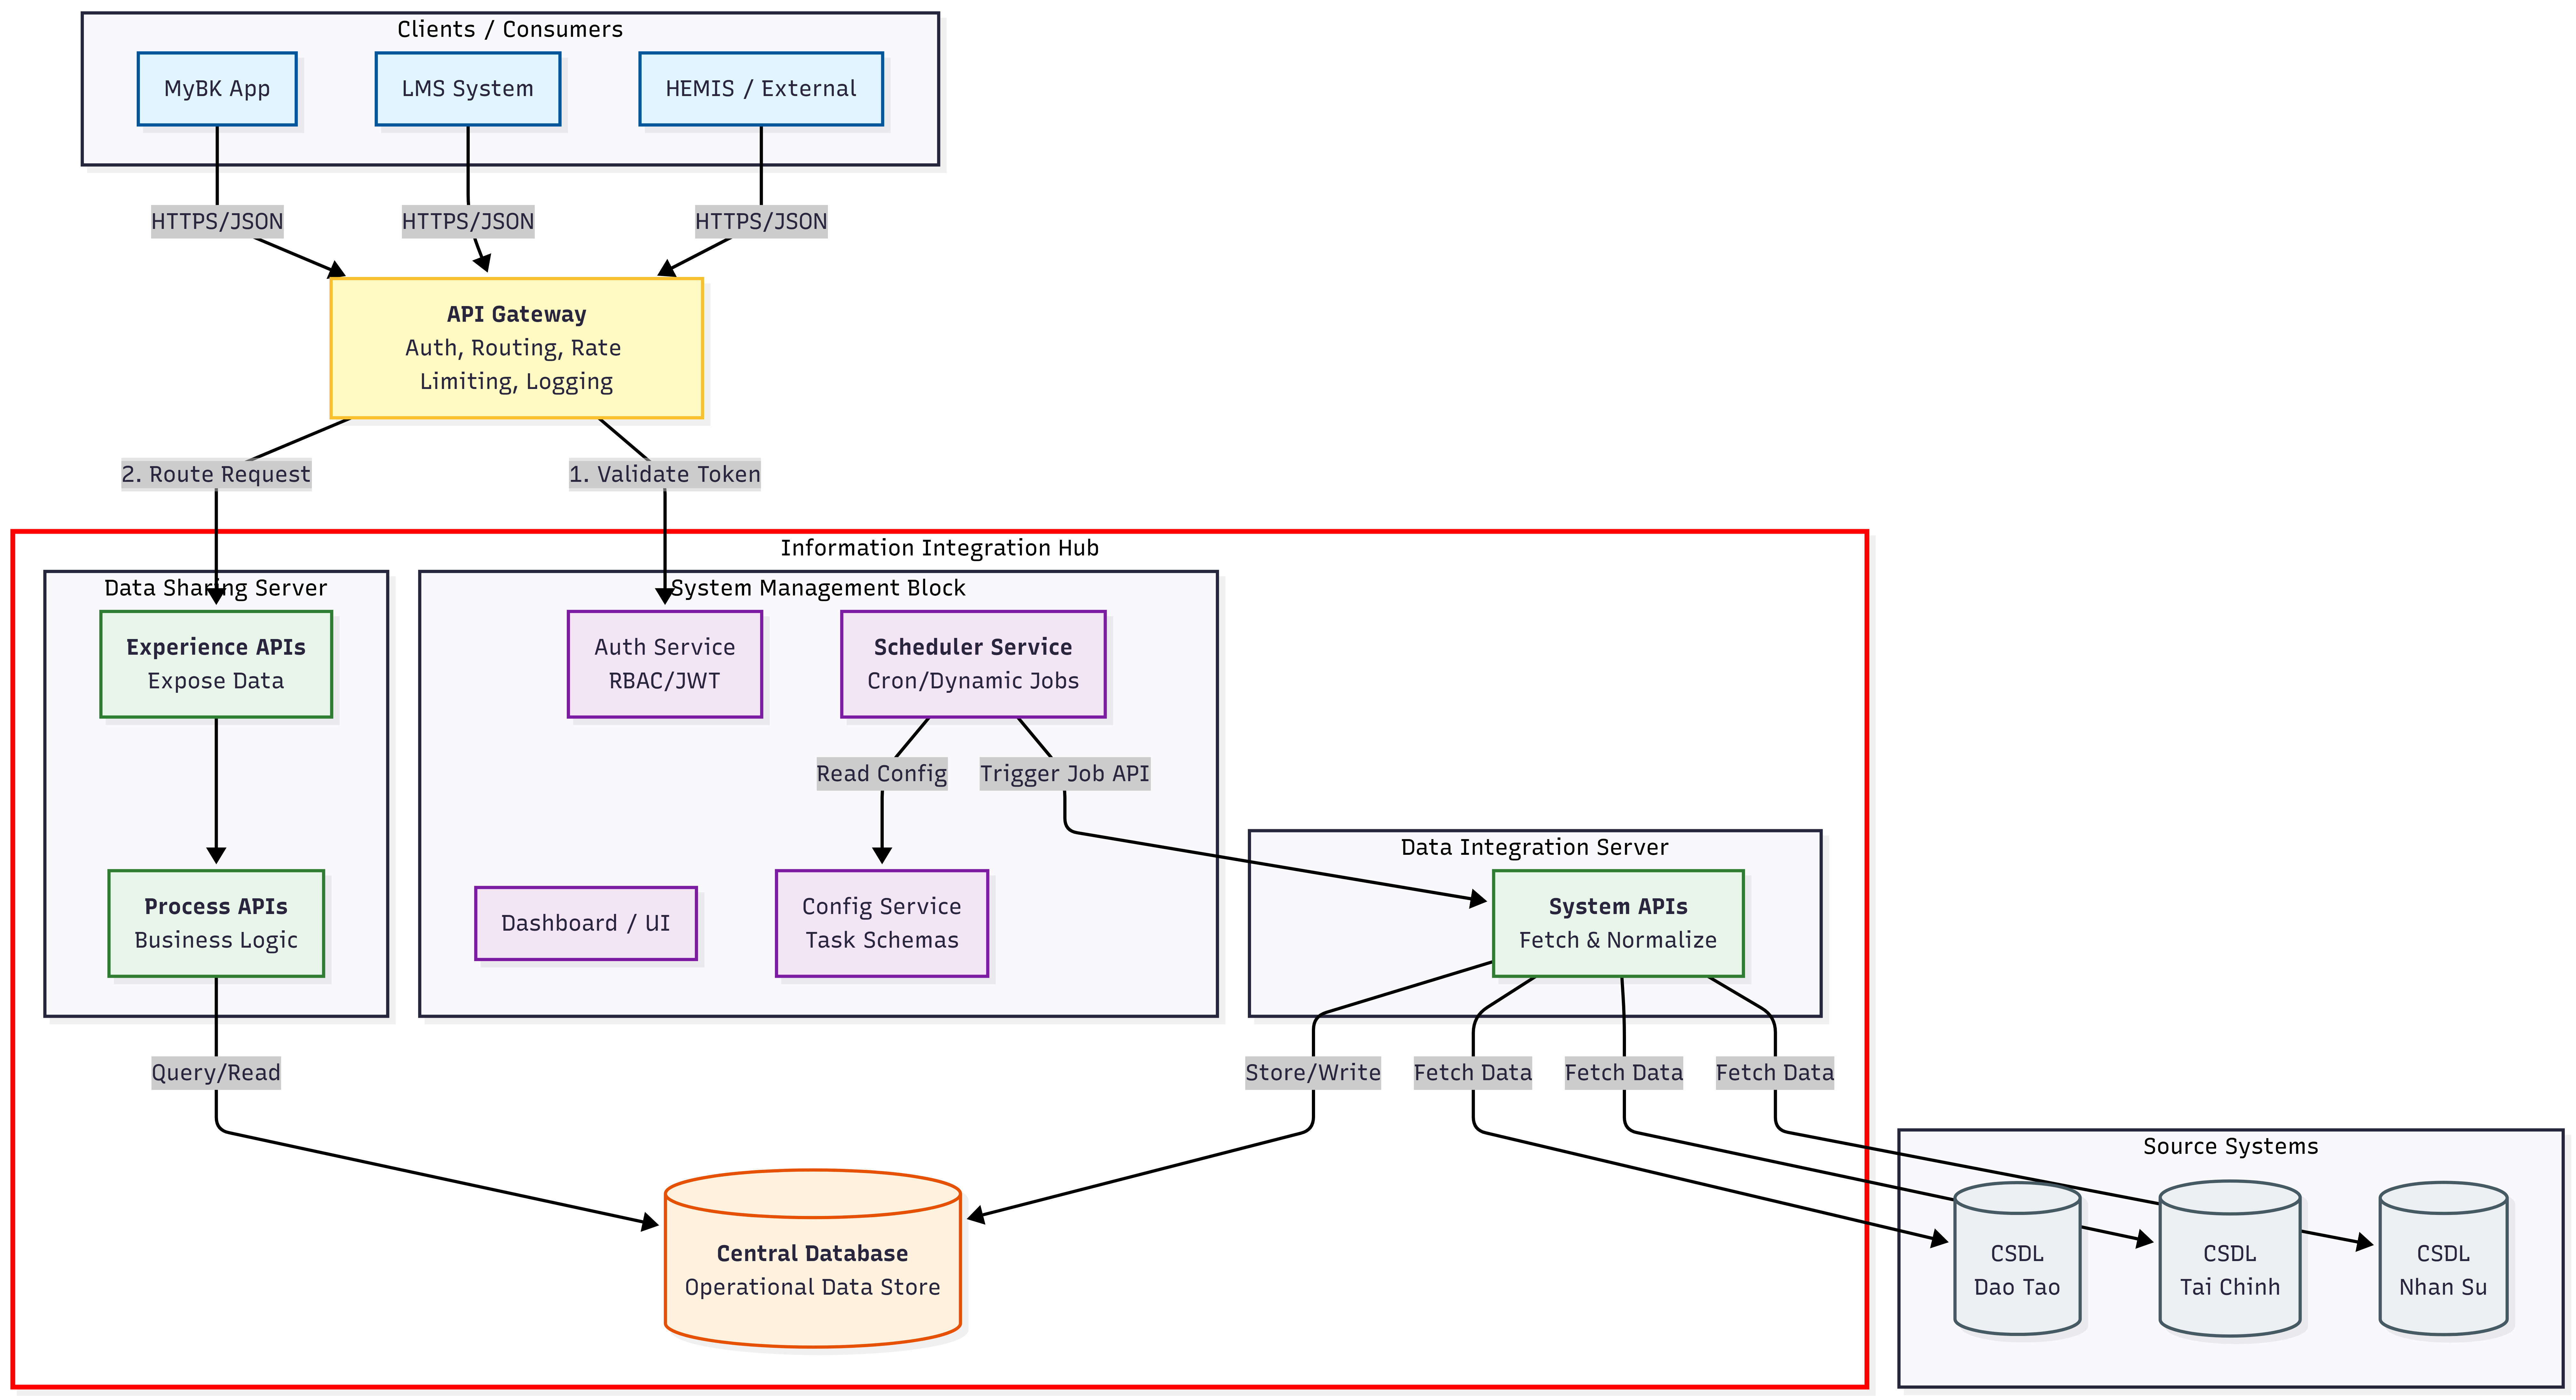
\includegraphics[width=\textwidth]{graphics/overview.png} 
    \caption{Sơ đồ kiến trúc tổng thể của Trục tích hợp dữ liệu}
    \label{fig:architecture_diagram}
\end{figure}

\section{Giải thích chi tiết các thành phần}
Kiến trúc được chia thành các khối thành phần chính, mỗi khối có một vai trò và trách nhiệm riêng biệt, tuân thủ theo mô hình API-led Connectivity ba lớp.

\subsection{Các hệ thống nguồn (Data Sources)}
Đây là tập hợp các cơ sở dữ liệu và hệ thống nghiệp vụ hiện có trong trường, chứa đựng các dữ liệu gốc cần được tích hợp. Mỗi hệ thống này sẽ cung cấp dữ liệu thông qua một lớp API riêng để đảm bảo tính an toàn và sự tách biệt, thay vì cho phép kết nối trực tiếp vào cơ sở dữ liệu.

\subsection{Trục tích hợp thông tin (Information Integration Hub)}
Đây là trái tim của toàn bộ hệ thống, được bao bọc bởi đường viền màu đỏ trong sơ đồ. Nó bao gồm các thành phần con sau:

\subsubsection{Máy chủ Tích hợp Dữ liệu (Data Integration Server)}
Thành phần này chịu trách nhiệm cho luồng dữ liệu đầu vào (ingestion flow), hiện thực hóa lớp \textbf{System API}:
\begin{itemize}
    \item \textbf{System API:} Đây là tập hợp các API nội bộ, có nhiệm vụ kết nối đến các API của hệ thống nguồn để trích xuất dữ liệu thô. Vai trò của nó là thu thập và trừu tượng hóa các hệ thống lõi, tạo ra một cách thức truy cập dữ liệu nhất quán.
    \item Sau khi trích xuất, máy chủ này sẽ thực hiện các bước biến đổi dữ liệu cơ bản (ETL/ELT) và nạp (stores) dữ liệu đã được làm sạch, chuẩn hóa vào Kho dữ liệu trung tâm.
\end{itemize}

\subsubsection{Máy chủ Chia sẻ Dữ liệu (Data Sharing Server)}
Thành phần này chịu trách nhiệm cho luồng dữ liệu đầu ra (query flow), hiện thực hóa hai lớp \textbf{Process API} và \textbf{Experience API}:
\begin{itemize}
    \item \textbf{Process API:} Lớp này chứa các logic nghiệp vụ phức tạp. Nó thực hiện truy vấn (queries) đến Kho dữ liệu trung tâm, kết hợp và tổng hợp thông tin để tạo ra các thực thể dữ liệu có giá trị nghiệp vụ cao.
    \item \textbf{Experience API:} Lớp trên cùng, có nhiệm vụ trả về các dữ liệu đã được xử lý bởi Process API ra cho các ứng dụng người dùng cuối. Các API ở lớp này được thiết kế tối ưu cho từng trải nghiệm cụ thể (ví dụ: API cho ứng dụng di động sẽ chỉ trả về những thông tin cần thiết nhất để tối ưu tốc độ).
\end{itemize}

\subsubsection{Kho dữ liệu trung tâm (Central Data Store)}
Đây là nơi lưu trữ dữ liệu đã được tích hợp và hợp nhất từ tất cả các nguồn. Nó đóng vai trò là cơ sở dữ liệu duy nhất cho toàn bộ các ứng dụng trong trường.

\subsection{Cổng API (API Gateway)}
API Gateway là cổng vào duy nhất cho tất cả các yêu cầu từ bên ngoài (MyBK, LMS, HEMIS) đến hệ thống. Nó chịu trách nhiệm:
\begin{itemize}
    \item \textbf{Xác thực (Authenticating):} Kiểm tra danh tính của người dùng/ứng dụng gọi đến.
    \item \textbf{Định tuyến (Routing):} Chuyển tiếp yêu cầu hợp lệ đến Experience API tương ứng trên Máy chủ Chia sẻ Dữ liệu.
    \item \textbf{Kiểm soát (Validating):} Áp dụng các chính sách bảo mật, giới hạn tần suất truy cập (rate limiting) để bảo vệ hệ thống.
\end{itemize}
\begin{figure}
    \centering
    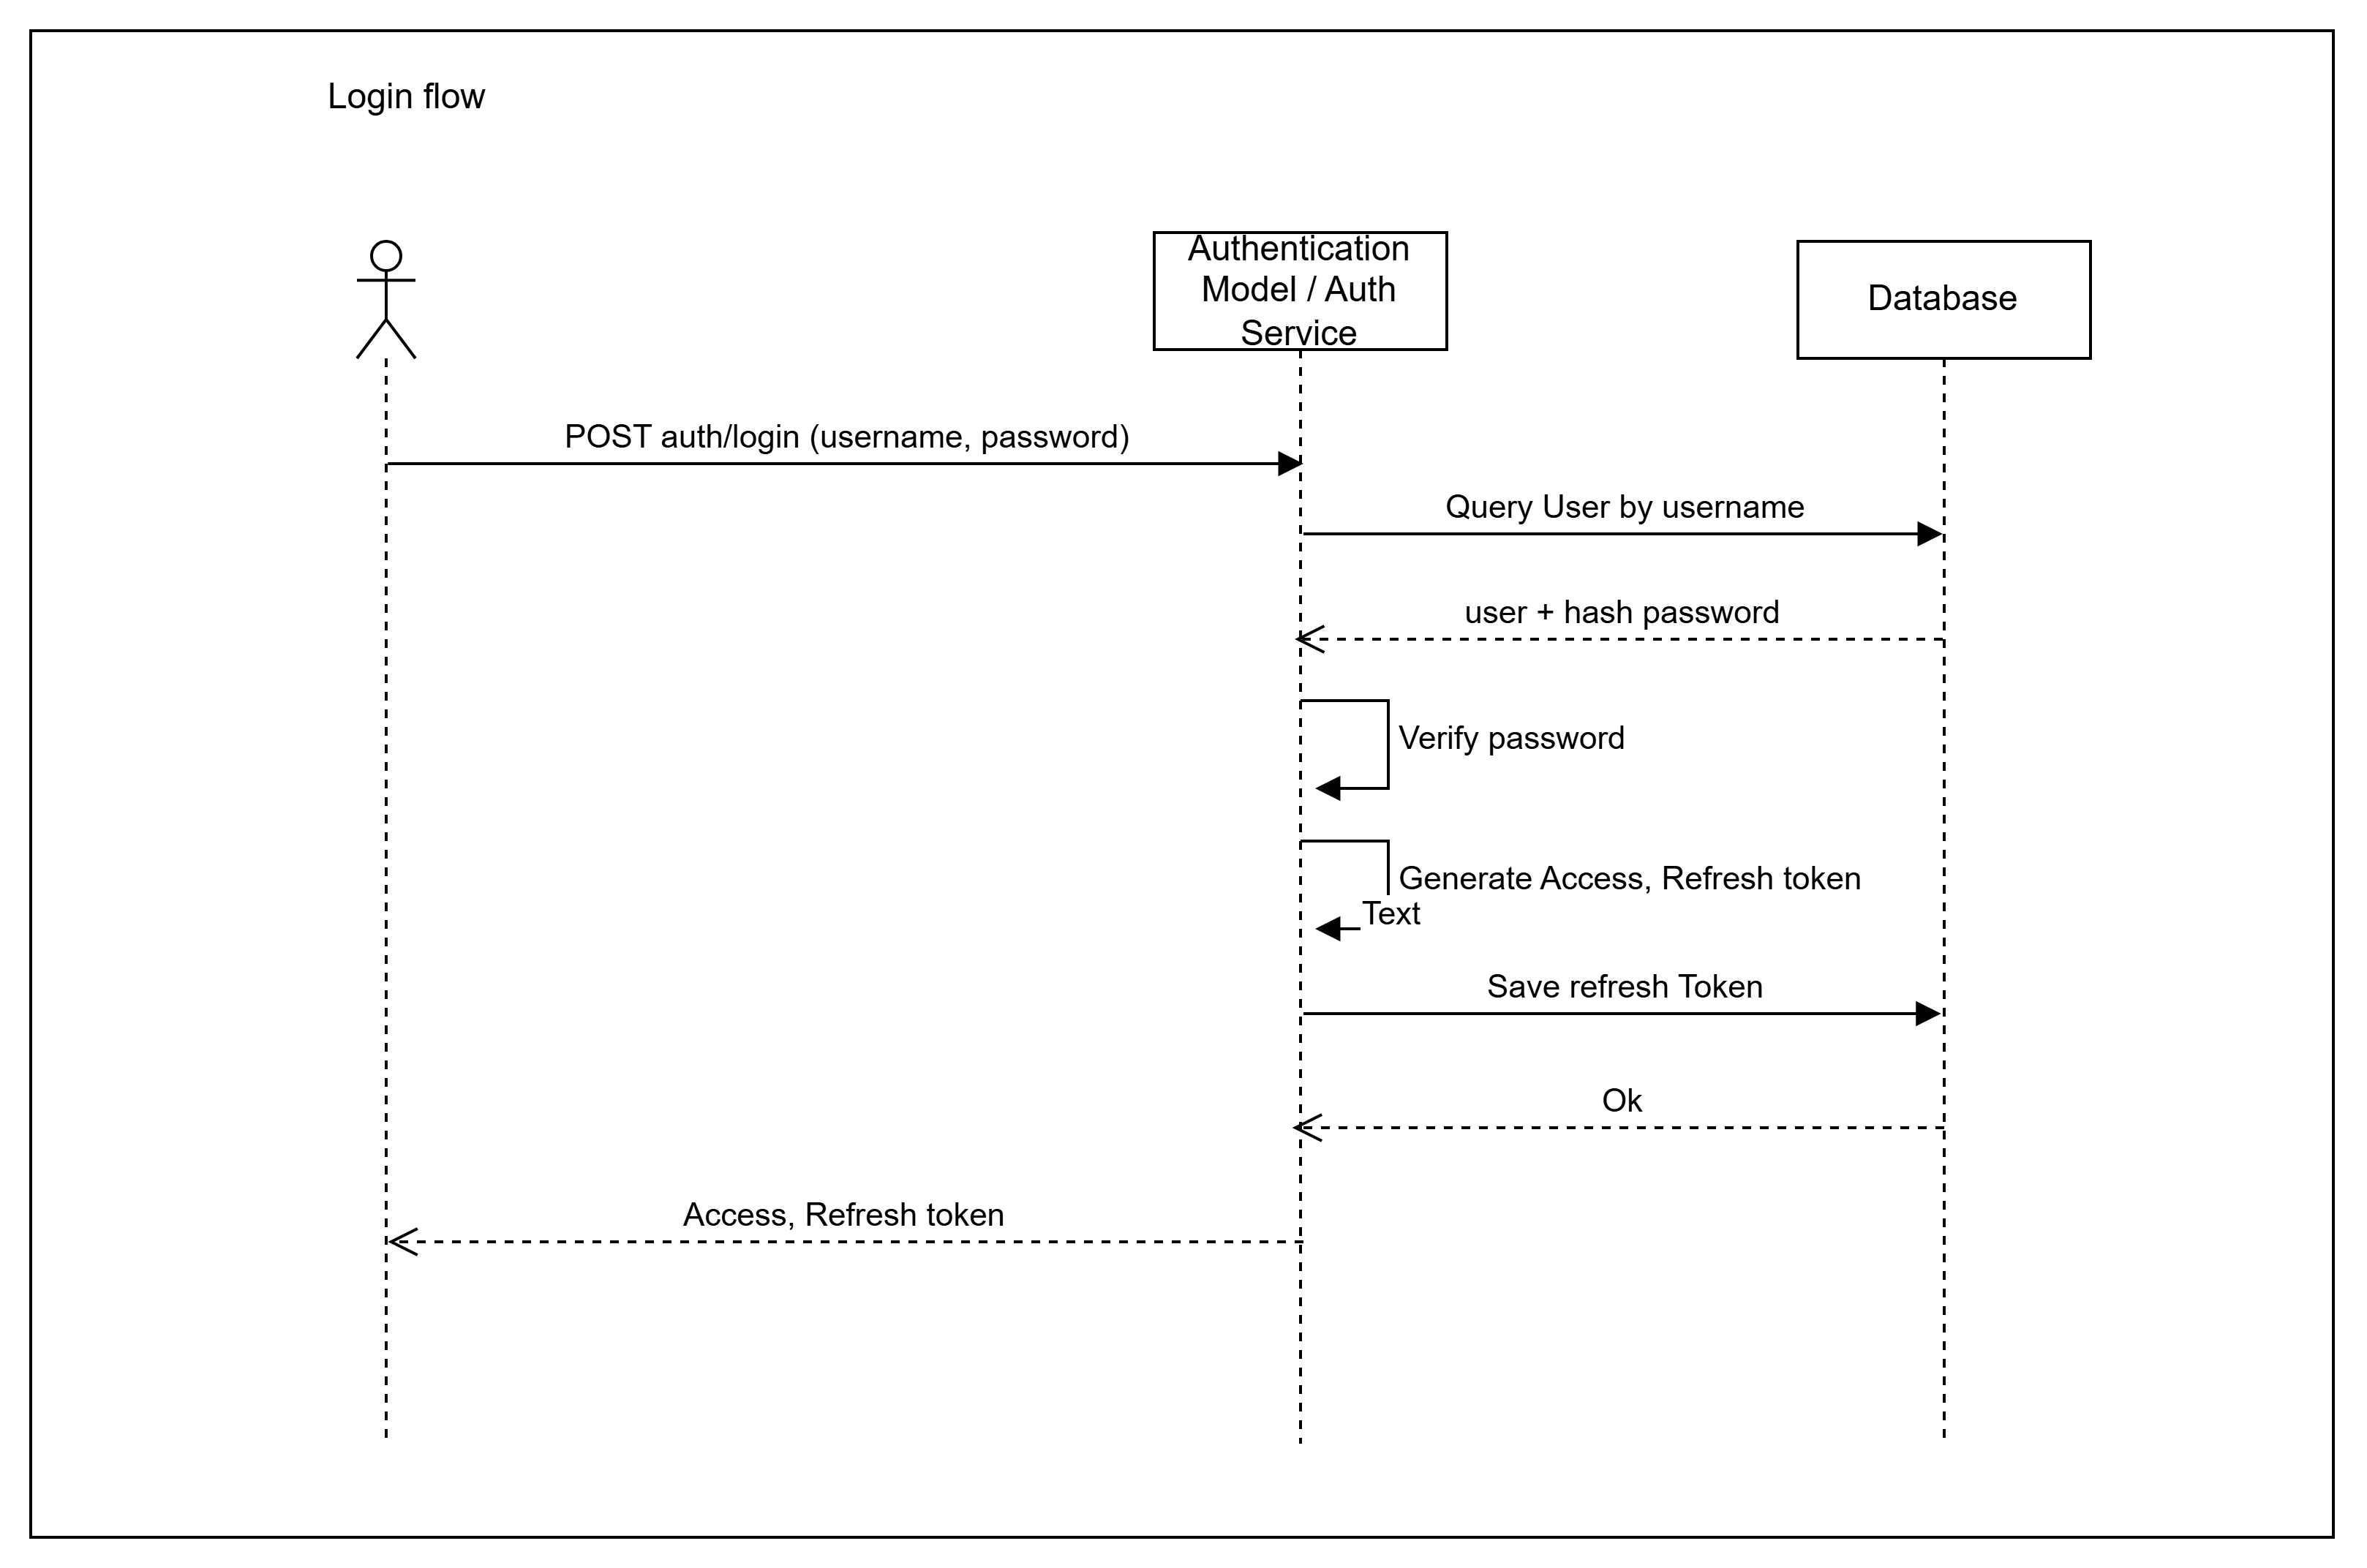
\includegraphics[width=1\linewidth]{graphics/logon_flow.png}
    \caption{Login Flow cho hệ thống}
\end{figure}

\subsection{Thiết kế chi tiết Module Quản lý Hệ thống}
Module Quản lý Hệ thống (System Management) là thành phần cốt lõi đảm bảo an ninh, quản trị và khả năng kiểm soát cho toàn bộ Trục tích hợp dữ liệu. Thay vì chỉ là một giao diện Dashboard đơn thuần, nó bao gồm một dịch vụ Xác thực và Phân quyền (Authentication and Authorization - Auth Service) mạnh mẽ, được thiết kế theo mô hình minh họa trong Hình \ref{fig:auth_flow}.

\subsubsection{Luồng Xác thực (Flow)}

Xác thực là quá trình xác minh danh tính của một người dùng hoặc một hệ thống. Luồng xử lý được thực hiện như sau:
\begin{enumerate}
    \item \textbf{Yêu cầu đăng nhập:} Người dùng (User) gửi thông tin định danh (ví dụ: username và password) đến ứng dụng backend (NestJS).
    \item \textbf{Xác minh thông tin:} Ứng dụng backend truy vấn vào Cơ sở dữ liệu (DataBase), cụ thể là bảng \texttt{Users}, để kiểm tra tính hợp lệ của thông tin đăng nhập.
    \item \textbf{Tạo và trả về JWT:} Nếu thông tin hợp lệ, hệ thống sẽ tạo ra một chuỗi JSON Web Token (JWT). JWT này là một chuỗi được mã hóa, chứa các thông tin (claims) về người dùng như ID, vai trò (role), và thời gian hết hạn. Token này sau đó được gửi về cho client (người dùng).
\end{enumerate}
Việc sử dụng JWT giúp cho hệ thống trở nên "stateless" (phi trạng thái), vì mọi thông tin cần thiết cho các phiên làm việc sau này đều được lưu trữ an toàn ngay trên client, giảm tải cho máy chủ.

\begin{figure}[!htp]
    \centering
    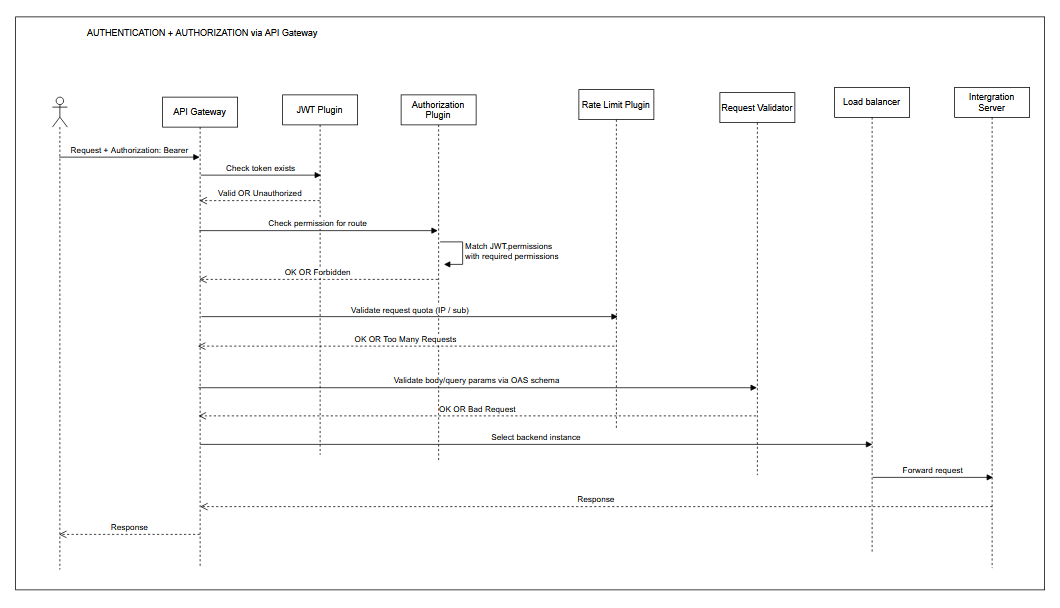
\includegraphics[width=\textwidth]{graphics/authentication_flow.png}
    \label{fig:auth_flow}
    \caption{Luồng xử lý Xác thực của hệ thống}
\end{figure}

\subsubsection{Luồng Phân quyền (Authorization Flow)}
Phân quyền là quá trình quyết định xem một người dùng đã được xác thực có quyền thực hiện một hành động cụ thể hay không. Quá trình này diễn ra ở mọi yêu cầu truy cập tài nguyên sau khi người dùng đã đăng nhập thành công:
\begin{enumerate}
    \item \textbf{Gửi yêu cầu kèm JWT:} Client gửi mỗi yêu cầu lên máy chủ, đính kèm JWT trong phần Header (thường là `Authorization: Bearer <token>`).
    \item \textbf{Xác thực Token:} API Gateway hoặc một lớp middleware trong ứng dụng NestJS sẽ chặn yêu cầu lại, giải mã và xác thực chữ ký của JWT để đảm bảo token là hợp lệ và chưa bị sửa đổi.
    \item \textbf{Kiểm tra quyền hạn (RBAC):} Sau khi xác thực token thành công, hệ thống sẽ thực hiện Phân quyền dựa trên mô hình \textbf{Role-Based Access Control (RBAC)}.
    \begin{itemize}
        \item Hệ thống đọc thông tin \textbf{Vai trò (Role)} của người dùng được đính kèm trong JWT (ví dụ: "Giảng viên", "Sinh viên", "Quản trị viên").
        \item Dựa trên Vai trò đó, hệ thống truy vấn vào cơ sở dữ liệu để xác định danh sách các \textbf{Quyền (Permissions)} mà vai trò đó sở hữu. Ví dụ, vai trò "Giảng viên" có quyền "Xem danh sách lớp học của mình", "Nhập điểm", nhưng không có quyền "Sửa học phí".
        \item Hệ thống so sánh quyền yêu cầu của hành động với danh sách quyền mà người dùng có. Nếu phù hợp, yêu cầu được chấp nhận; nếu không, yêu cầu bị từ chối.
    \end{itemize}
\end{enumerate}

\begin{figure}[!htp]
    \centering
    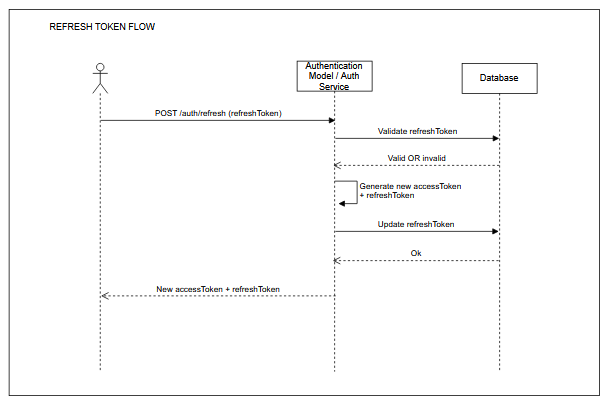
\includegraphics[width=\textwidth]{graphics/refresh_token.png} 
    \caption{Luồng xử lý refresh token của hệ thống}
    \label{fig:refresh_token}
\end{figure}

\newpage
\subsubsection{Cấu trúc Cơ sở dữ liệu cho RBAC}
Để hiện thực hóa mô hình RBAC, cơ sở dữ liệu được thiết kế với các bảng chính sau:
\begin{itemize}
    \item \textbf{Users:} Lưu trữ thông tin định danh của người dùng (username, password đã được hash, thông tin cá nhân...).
    \item \textbf{Roles:} Định nghĩa các vai trò trong hệ thống.
\end{itemize}
Mối quan hệ nhiều-nhiều giữa chúng được thể hiện qua các bảng trung gian (không có trong sơ đồ nhưng là một phần của thiết kế):
\begin{itemize}
    \item \textbf{user\_roles:} xạ người dùng nào có vai trò nào.
\end{itemize}
Cấu trúc này mang lại sự linh hoạt tối đa, cho phép người quản trị có thể dễ dàng tạo ra các vai trò mới hoặc thay đổi quyền hạn của một vai trò mà không cần can thiệp vào mã nguồn của ứng dụng, thông qua giao diện Dashboard của Module Quản lý Hệ thống.

\begin{figure}[!htp]
    \centering
    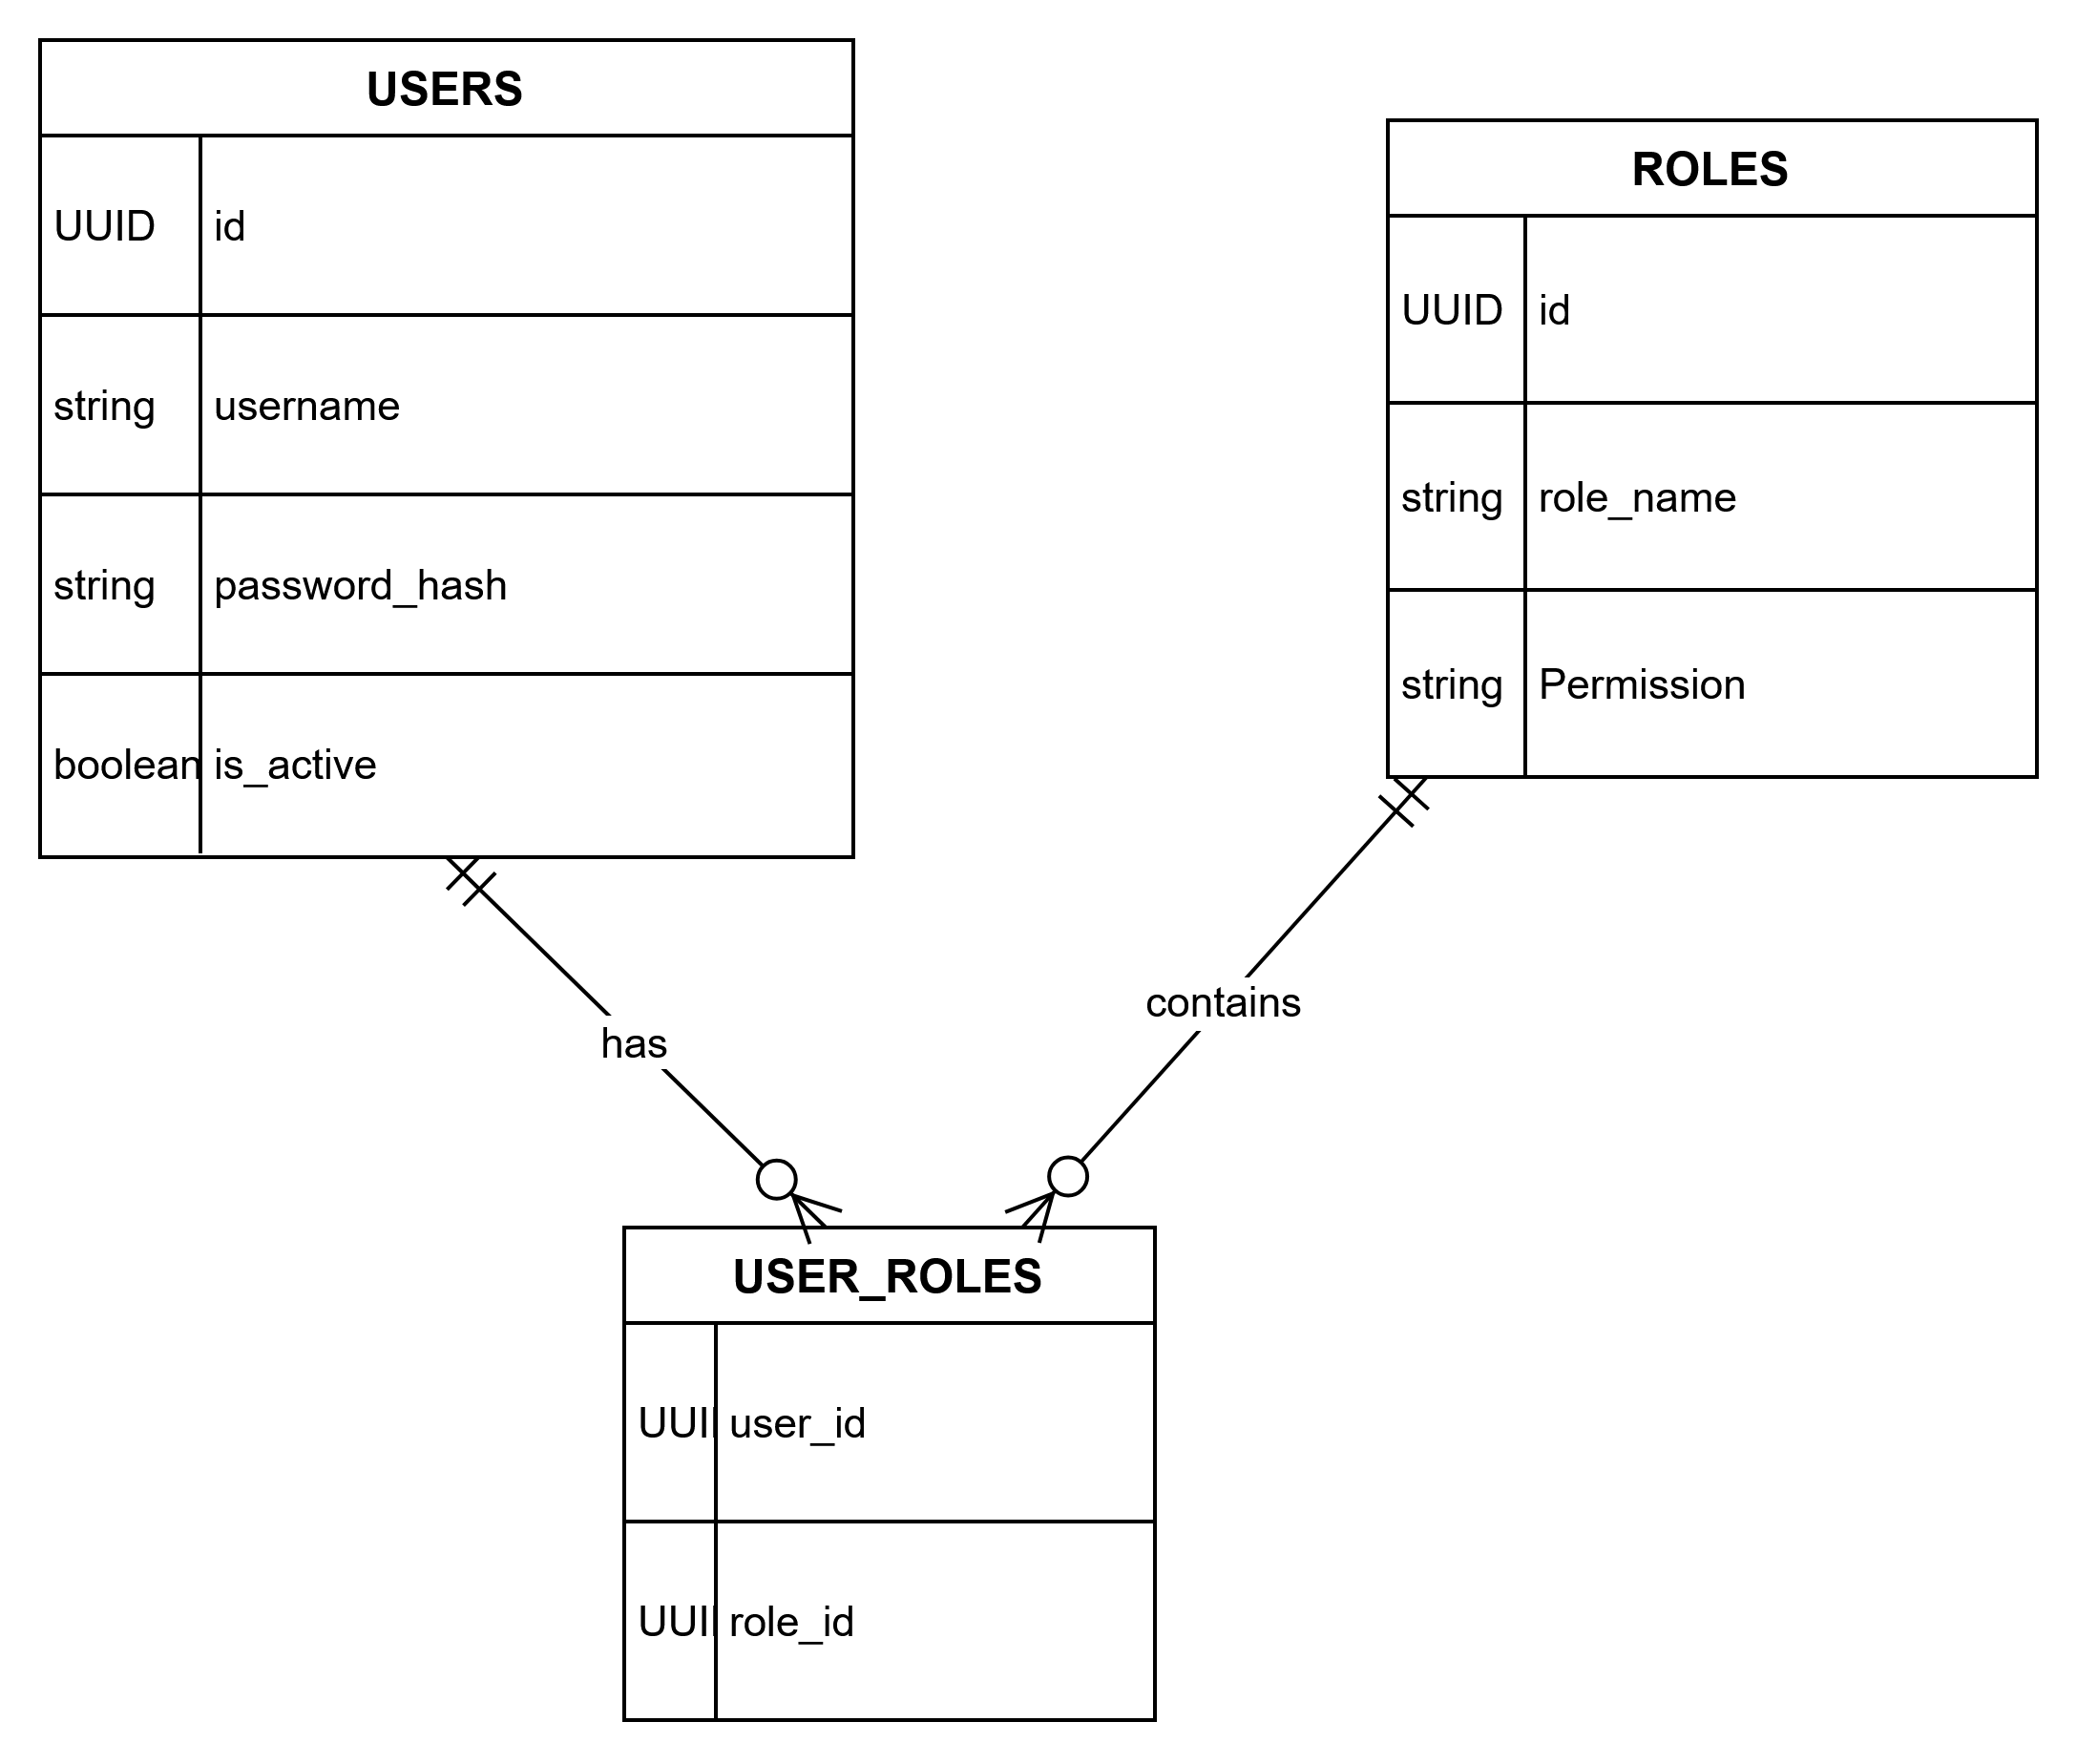
\includegraphics[width=12cm]{graphics/RBAC.png} 
    \caption{RBAC}
    \label{fig:rbac}
\end{figure}

